\section*{Question 2}

\subsection*{Newton-Raphson}

Utilisons le théorème $3.10$ énoncé à la question 1.
Dans notre cas, on voit aisément que $J_G(y) = W_{\bot}^*AW_{\bot} - w^*AwI - (yw^*AW_{\bot}+Iw^*AW_{\bot}y) $ est continu en $s$ ($I$ est la matrice identité de taille $n-1$).

On peut étendre le théorème $3.10$ avec des hypothèses plus forte sur la jacobienne : 

Si, de plus, il existe une constante $\alpha > 0$ telle que la condition de Lipschitz est satisfaite
$$||DF(x) - DF(s)|| \leq \alpha || x - s||, \forall x \in \Omega,$$
alors l'ordre de convergence est au moins 2. 

Dans notre cas, en utilisant l'inégalité de Cauchy et l'inégalité triangulaire, on obtient que : 
\begin{eqnarray}
||DG(x) - DG(s)|| &=& ||W_{\perp}^{*} A W_{\perp}- w^{*} A wI - (xw^*AW_{\bot}+Iw^*AW_{\bot}x) - W_{\perp}^{*} A W_{\perp}+ w^{*} A wI + (sw^*AW_{\bot}+Iw^*AW_{\bot}s) || \\
||DG(x) - DG(s)|| &=&  ||(sw^*AW_{\bot}+Iw^*AW_{\bot}s) - (xw^*AW_{\bot}+Iw^*AW_{\bot}x) || \\
 ||DG(x) - DG(s)|| &\leq & (||w^*AW_{\bot}|| + || Iw^*AW_{\bot} ||) || x-s ||
\end{eqnarray}
Par identification on a $\alpha = ||w^*AW_{\bot}|| + || Iw^*AW_{\bot} || \geq 0$, et donc la condition de Lipschitz sur $DG(x)$ est satisfaite.On conclut qu'on a bien un ordre de convergence d'au moins 2 pour la méthode de Newton appliquée à la fonction $G$.

\subsection*{Rayleigh symétrique}
On peut voir la méthode de Rayleigh comme une méthode de la puissance avec un "shift" variable (mis a jour à chaque itération). En d'autre mots, elle définie la méthode itérative suivante : 
$$x_{k+1} = \left(  A- \frac{x^*Ax}{x^*x}  \right)^{-1} x_k.  $$
\textbf{Proposition 4.4} Soit $A = A^*$ $ \in \mathbb{C}^{n\times n}$. L'itération du quotient de Rayleigh pour $A$ converge vers une direction propre de $A$ pour presque tout itéré initial. Lorsque la suite des itérés converge vers une direction propre, la convergence est cubique. 

Il faut maintenant préciser ce \textit{pour presque tout itéré initial}. Supposons que $A$ est diagonalisable et faisons un changement de variable afin d'exprimer $x$ dans la base formée par les vecteurs propres de $A$. Nommons le $x$ après changement de variables $x'$. Soit $Q$ la matrice dont les colonnes sont les vecteurs propres de $A$ et $D$ la matrice diagonale des valeurs propres de $A$. On utilise le théorème spectrale et le fait que $A$ et $(A-\mu I)^{-1}$ possèdent les mêmes vecteurs propres pour réécrire l'itération : 
\begin{eqnarray}
Qx_{k+1}' & = &(Q D Q^T - \frac{x_k'^* D x_k}{x_k'^* x_k})^{-1} Qx_{k}'\\
Qx_{k+1}' & = & Q(D-\frac{x_k'^* D x_k}{x_k'^* x_k})^{-1}Q^T Qx_k'\\
x_{k+1}' & = & \underbrace{(D-\frac{x_k'^* D x_k}{x_k'^* x_k})^{-1}}_{\text{matrice diagonale}} x_k'
\end{eqnarray}
Supposons qu'on souhaite converger vers le vecteur propres dominant $v_1$, autrement dit on souhaite que $lim_{k\rightarrow \infty} x_k' = [1 0 \cdots 0]^T$. Pour que cela soit possible, il faut que $x_0$ ait sa composante dans la direction $v_1$ non nulle ($x_0'^* v_1 \neq 0$). 

Vérifions maintenant de manière numérique les résultats théoriques obtenus. Prenons par exemple la matrice symétrique $A$ : 

$$ A = \left[
\begin{array}{ccc}
  2 & 4 & 6  \\
  4 & 2 & 1 \\
  6 & 1 & 2 \\
\end{array}
\right]$$

En utilisant la fonction $eigs$ de \textit{Matlab}, on sait que les valeurs propres de $A$ sont : 
   \begin{eqnarray*}
   \lambda_1 &=& 9.6965\\
   \lambda_2 &=& 1.0796 \\
   \lambda_3 &=& -4.7762
   \end{eqnarray*}

En appliquant l'itération du quotient de Rayleigh symétrique implémentée par nos soins pour un $x_0$ tel que : 
$$ x_0 = \left[
\begin{array}{c}
  \frac{1}{\sqrt{3}}  \\
  \frac{1}{\sqrt{3}} \\
  \frac{1}{\sqrt{3}} \\
\end{array}
\right]$$
 et pour $\mu_0 = 1000$ (la valeur propre la plus "proche" est donc 9.696530) , on obtient : 
$$\begin{array}{ccc}
  itération & erreur & \mu  \\
  1 &  990.658295   & \underline{9}.341705  \\
  2 &   0.354404   &  \underline{9.696}109\\
  3 &  0.000421  & \underline{9.696530} \\
  4 &  0.000000  & \underline{9.696530} \\
\end{array}$$

Ce qui correspond bien à la théorie. En effet, à chaque itération on gagne bien 3 chiffres significatifs comme l'illustrent l'erreur (définie comme la différence entre les $\mu_k$ à chaque itération) et les chiffres soulignés qui représentent les chiffres significatifs du $\mu_k$.

On considère maintenant un itéré initial qui n'a pas de composante dans la direction du vecteur propre  

$$ v_1 = \left[
\begin{array}{c}
  0.6834  \\
   0.4317 \\
   0.5888 \\
\end{array}
\right], \text{ t.q. } Av_1 = \lambda_1 v_1,$$

par exemple  :

$$ x_0 = \left[
\begin{array}{c}
  1  \\
  0 \\
  -1.1606\\
\end{array}
\right]$$

Lorsqu'on applique l'itération, on ne converge effectivement plus vers $\lambda_1$ mais vers $\lambda_3$. Le \textit{pour presque tout itéré initial} est donc confirmé.

\textbf{je sais ces image et explications puent pour l'instant, je les mets parce que j'ai fait le script et tout mais en soit hesitez pas à modifier et vu qu'elles vont peut etre disparaitre du rapport ca me soule d'écrire un roman pour l'expliquer nickel :p}

L'image suivante illustre les valeurs propres (sur l'axe des z, 9.6965 1.0796 -4.7762 ) vers lesquelles on converge pour différents vecteurs propres initiaux $x_0$ (représentés par les points 1, 2 ou 3 sur l'axe des x, cf. code pour savoir leur valeurs exactes) et pour différents $\mu$ initiaux (de -10 à 10 sur l'axe des y).

\begin{figure}
  \centering
  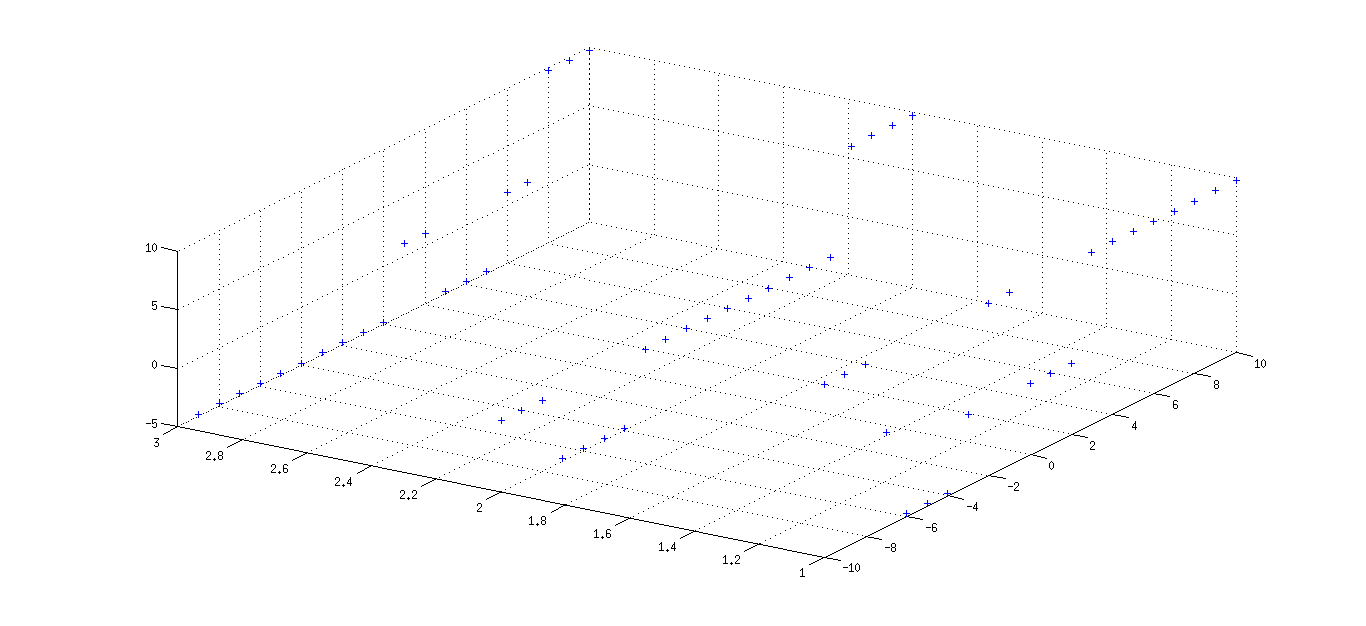
\includegraphics[width=15cm]{RaySym.png}
  \caption{Graphe représentant les valeurs propres vers lesquelles on converge pour différents $x_0$ et $mu$}
  \label{fig:RaySym}
\end{figure}
\subsection*{Rayleigh asymétrique}

